\documentclass[a4paper, 14pt]{article}
\usepackage[utf8]{inputenc}
\usepackage[russian]{babel}
\usepackage{graphicx}
\usepackage{listings}
\usepackage{color}
\usepackage{amsmath}
\usepackage{pgfplots}
\usepackage{url}
% подключаем hyperref (для ссылок внутри  pdf)
\usepackage[unicode, pdftex]{hyperref}
\usepackage[T2A]{fontenc}
\usepackage[utf8]{inputenc}
\lstset{tabsize=2,
    breaklines,
    columns=fullflexible,
    flexiblecolumns,
    numbers=left,
    keepspaces=true,
    numberstyle={\footnotesize},
    extendedchars=\true
}
\lstdefinelanguage{MyC}{
  language=C++,
  ndkeywordstyle=\color{darkgray}\bfseries,
  identifierstyle=\color{black},
  morecomment=[n]{/**}{*/},
  commentstyle=\color{blue}\ttfamily,
  stringstyle=\color{red}\ttfamily,
  morestring=[b]",
  showstringspaces=false,
  morecomment=[l][\color{gray}]{//},
  keepspaces=true,
  escapechar=\%,
  %texcl=⟨true|false⟩
}
%\usepackage[russian,russian,english]{babel}
\frenchspacing                    % ставим пробелы в соответствии с французским стилем
\DeclareGraphicsExtensions{.pdf,.png,.jpg,.svg}
\usepackage{titlesec}
\usepackage[russian]{babel}
\usepackage{algpseudocode}
\usepackage{caption}
\usepackage{setspace}
\usepackage[linesnumbered,boxed]{algorithm2e}
\DeclareCaptionFont{white}{\color{white}} %% это сделает текст заголовка белым
%% код ниже нарисует серую рамочку вокруг заголовка кода.

\linespread{1}

\DeclareCaptionFormat{listing}{\colorbox{gray}{\parbox{\textwidth}{#1#2#3}}}
\captionsetup[lstlisting]{format=listing,labelfont=white,textfont=white} 

\begin{document}
	\begin{titlepage}
		\begin{center}
			\begin{LARGE}
				Отчет по лабораторной работе №2\\
					по курсу "Анализ алгоритмов"\\
					по теме "Сортировки"
			\end{LARGE}
		
			\begin{Large}
				\vspace{10cm}
				Студент: Доктор А.А. ИУ7-53\\
					Преподаватель: Волкова Л.Л.,
								   Строганов Ю.В.\\
				
				\vspace{5cm}2018 г.				   
			\end{Large}
			
		\end{center}
		 
	\end{titlepage}

\tableofcontents
	
\newpage
\section*{Введение}
\addcontentsline{toc}{section}{Введение}
\hspace{1cm}Алгоритм сортировки — это алгоритм для упорядочивания элементов в списке. В случае, когда элемент списка имеет несколько полей, поле, служащее критерием порядка, называется ключом сортировки. На практике в качестве ключа часто выступает число, а в остальных полях хранятся какие-либо данные, никак не влияющие на работу алгоритма.
Алгоритмы сортировки оцениваются по скорости выполнения и эффективности использования памяти:

\begin{doublespace}
\large
\textbf{Оценка алгоритма сортировки}
\normalsize
\end{doublespace}

Ниже приведены параметры оценки эффективности алгоритма \cite{alg_params}.
\begin{enumerate}
\item Время — параметр, характеризующий быстродействие алгоритма. Называется также вычислительной сложностью. Для упорядочения важны худшее, среднее и лучшее поведение алгоритма в терминах мощности входного множества A. Если на вход алгоритму подаётся множество A, то обозначим n = |A|. Для типичного алгоритма хорошее поведение — это O(n log n) и плохое поведение — это O(n2). Идеальное поведение для упорядочения — O(n). Алгоритмы сортировки, использующие только абстрактную операцию сравнения ключей всегда нуждаются по меньшей мере в сравнениях. Тем не менее, существует алгоритм сортировки Хана (Yijie Han) с вычислительной сложностью O(n log log n log log log n), использующий тот факт, что пространство ключей ограничено (он чрезвычайно сложен, а за О-обозначением скрывается весьма большой коэффициент, что делает невозможным его применение в повседневной практике). Также существует понятие сортирующих сетей. Предполагая, что можно одновременно (например, при параллельном вычислении) проводить несколько сравнений, можно отсортировать n чисел за O(log2 n) операций. При этом число n должно быть заранее известно.
\item Память — ряд алгоритмов требует выделения дополнительной памяти под временное хранение данных. Как правило, эти алгоритмы требуют O(log n) памяти. При оценке не учитывается место, которое занимает исходный массив и независящие от входной последовательности затраты, например, на хранение кода программы (так как всё это потребляет O(1)). Алгоритмы сортировки, не потребляющие дополнительной памяти, относят к сортировкам на месте.
\item Устойчивость - устойчивая сортировка не меняет взаимного расположения равных элементов. Такое свойство может быть очень полезным, если они состоят из нескольких полей, 
\item Естественность поведения - эффективность метода при обработке уже отсортированных, или частично отсортированных данных. Алгоритм ведет себя естественно, если учитывает эту характеристику входной последовательности и работает лучше.

\end{enumerate}

Еще одним важным свойством алгоритма является его сфера применения. Здесь основных позиций две:
\begin{enumerate}
\item внутренние сортировки работают с данным в оперативной памяти с произвольным доступом;
\item внешние сортировки упорядочивают информацию, расположенную на внешних носителях. Это накладывает некоторые дополнительные ограничения на алгоритм:
доступ к носителю осуществляется последовательным образом: в каждый момент времени можно считать или записать только элемент, следующий за текущим
объем данных не позволяет им разместиться в ОЗУ
Кроме того, доступ к данным на носителе производится намного медленнее, чем операции с оперативной памятью.
\end{enumerate}

Данный класс алгоритмов делится на два основных подкласса:
\begin{enumerate}
\item Внутренняя сортировка оперирует с массивами, целиком помещающимися в оперативной памяти с произвольным доступом к любой ячейке. Данные обычно сортируются на том же месте, без дополнительных затрат.

\item Внешняя сортировка оперирует с запоминающими устройствами большого объема, но с доступом не произвольным, а последовательным (сортировка файлов), т.е в данный момент мы 'видим' только один элемент, а затраты на перемотку по сравнению с памятью неоправданно велики . Это приводит к специальным методам сортировки, обычно использующим дополнительное дисковое пространство.
\end{enumerate}

\newpage
\section*{Задачи работы}

Выше я перечислил основные сортировки, существующие на сегодняшний день, однако в данной лабораторной я разберу лишь некоторые из них, а именно:

\begin{enumerate}
\item[1)] сортировка вставками(Insertion) с бинарным поиском;
\item[2)] терпеливая(patience) сортировка;
\item[2)] поразрядная LSD сортировка;
\end{enumerate}


\newpage
\section{Аналитическая часть}
\hspace{1cm}	В данном разделе приведено описание сортировок.
\subsection{Описание алгоритмов}
\begin{doublespace}

\large
\textbf{Сортировка вставками}
\normalsize
\end{doublespace}
Сортировка вставками (Insertion Sort) — это простой алгоритм сортировки, в котором элементы входной последовательности просматриваются по одному, и каждый новый поступивший элемент размещается в подходящее место среди ранее упорядоченных элементов. \cite{knut}

На вход алгоритма подаётся последовательность n чисел: $a_{1}$,$a_{2}$,...,$a_{n}$.
Сортируемые числа также называют ключами. Входная последовательность на практике представляется в виде массива с n элементами. На выходе алгоритм должен вернуть перестановку исходной последовательности $a'_{1}$,$a'_{2}$,...,$a'_{n}$, чтобы выполнялось следующее соотношение $a'_{1}$ \le $a'_{2}$ ... \le $a'_{n}$ \cite{korman}.

В начальный момент отсортированная последовательность пуста. На каждом шаге алгоритма выбирается один из элементов входных данных и помещается на нужную позицию в уже отсортированной последовательности до тех пор, пока набор входных данных не будет исчерпан. В любой момент времени в отсортированной последовательности элементы удовлетворяют требованиям к выходным данным алгоритма \cite{macconel}.

Данный алгоритм можно ускорить при помощи использования бинарного поиска для нахождения места текущему элементу в отсортированной части.


\begin{doublespace}
\large
\textbf{Терпеливая сортировка}
\normalsize
\end{doublespace}

Терпеливая сортировка (англ. patience sorting) — алгоритм сортировки с худшей сложностью O(n log n). Позволяет также вычислить длину наибольшей возрастающей подпоследовательности данного массива. Алгоритм назван по одному из названий карточной игры "Солитёр" — "Patience".

\begin{doublespace}
\large
Алгоритм
\normalsize
\end{doublespace}

Имеем массив source[0..n−1], элементы которого нужно отсортировать по возрастанию. Разложим элементы массива по стопкам: для того чтобы положить элемент в стопку, требуется выполнение условия — новый элемент меньше элемента, лежащего на вершине стопки; либо создадим новую стопку справа и сделаем наш элемент её вершиной. Используем жадную стратегию: каждый элемент кладётся в самую левую стопку из возможных, если же таковой нет, справа от существующих стопок создаётся новая. Для получения отсортированного массива сначала построим массив стопок, затем выполним n шагов (здесь и далее нумерация шагов начинается с единицы): на i-м шаге выберем из всех вершин стопок наименьшую, извлечём её и запишем в массив ans[0..n−1] на i-ю позицию.

Мы формируем новую стопку, когда встречаем элемент больший, чем вершины всех стопок, расположенных слева. В то же время стопки слева были созданы ранее, то есть элементы в них идут в исходной последовательности раньше текущего. Каждая стопка представляет собой убывающую последовательность, то есть длина НВП в пределах стопки равна единице, поэтому появление новой стопки можно понимать как увеличение длины наибольшей возрастающей подпоследовательности на единицу (изначально длина НВП равна единице). Поэтому длина наибольшей возрастающей подпоследовательности равна количеству стопок.

\begin{doublespace}
\large
Сложность
\normalsize
\end{doublespace}

Создадим список стеков для хранения стопок. При раскладывании элементов по стопкам для поиска самой левой подходящей стопки используем бинарный поиск. Соответственно, поиск самой левой стопки занимает O(log p), где p — количество стопок (стеков). Таким образом, временная сложность раскладывания по стопкам не превышает O(nlogn).

Для получения отстортированного массива используем бинарную кучу. На каждом шаге алгоритма необходимо извлечь из кучи стек с минимальной вершиной за O(log p), где p — количество стеков в куче. Снять вершину выбранного стека и вернуть его в кучу за O(log p). Получение отсортированного массива займёт O(nlog n) времени. Получение наибольшей возрастающей подпоследовательности выполняется за O(n) по описанному выше алгоритму. Таким образом, алгоритм сортировки требует O(nlogn) времени в худшем случае и O(n) дополнительной памяти при любом раскладе.

\begin{doublespace}
\large
\textbf{Поразрядная сортировка}
\normalsize
\end{doublespace}

Поразрядная сортировка (англ. radix sort) — один из алгоритмов сортировки, использующих внутреннюю структуру сортируемых объектов.

\begin{doublespace}
\large
Алгоритм
\normalsize
\end{doublespace}

Исходно предназначен для сортировки целых чисел, записанных цифрами. Но так как в памяти компьютеров любая информация записывается целыми числами, алгоритм пригоден для сортировки любых объектов, запись которых можно поделить на «разряды», содержащие сравнимые значения. Например, так сортировать можно не только числа, записанные в виде набора цифр, но и строки, являющиеся набором символов, и вообще произвольные значения в памяти, представленные в виде набора байт.

Сравнение производится поразрядно: сначала сравниваются значения одного крайнего разряда, и элементы группируются по результатам этого сравнения, затем сравниваются значения следующего разряда, соседнего, и элементы либо упорядочиваются по результатам сравнения значений этого разряда внутри образованных на предыдущем проходе групп, либо переупорядочиваются в целом, но сохраняя относительный порядок, достигнутый при предыдущей сортировке. Затем аналогично делается для следующего разряда, и так до конца.

Так как выравнивать сравниваемые записи относительно друг друга можно в разную сторону, на практике существуют два варианта этой сортировки. Для чисел они называются в терминах значимости разрядов числа, и получается так: можно выровнять записи чисел в сторону менее значащих цифр (по правой стороне, в сторону единиц, least significant digit, LSD) или более значащих цифр (по левой стороне, со стороны более значащих разрядов, most significant digit, MSD).

\begin{doublespace}
\large
\textbf{LSD-сортировка (Least Significant Digit radix sort)}
\normalsize
\end{doublespace}

При LSD сортировке (сортировке с выравниванием по младшему разряду, направо, к единицам) получается порядок, уместный для чисел. Например: 1, 2, 9, 10, 21, 100, 200, 201, 202, 210. То есть, здесь значения сначала сортируются по единицам, затем сортируются по десяткам, сохраняя отсортированность по единицам внутри десятков, затем по сотням, сохраняя отсортированность по десяткам и единицам внутри сотен, и т. п.

В качестве примера рассмотрим сортировку чисел. Как говорилось выше, в такой ситуации в качестве устойчивой сортировки применяют сортировку подсчетом, так как обычно количество различных значений разрядов не превосходит количества сортируемых элементов. Ниже приведен псевдокод цифровой сортировки, которой подается массив A размера n m-разрядных чисел . Сам по себе алгоритм представляет собой цикл по номеру разряда, на каждой итерации которого элементы массива A размещаются в нужном порядке во вспомогательном массиве B. Для подсчета количества объектов, i-й разряд которых одинаковый, а затем и для определения положения объектов в массиве B используется вспомогательный массив C. Функция digit(x,i) возвращает i-й разряд числа x. Также считаем, что значения разрядов меньше k.

\begin{doublespace}
\large
\textbf{MSD-сортировка (Most Significant Digit radix sort)}
\normalsize
\end{doublespace}

При MSD сортировке (с выравниванием в сторону старшего разряда, налево), получается алфавитный порядок, который уместен для сортировки строк текста. Например «b, c, d, e, f, g, h, i, j, ba» отсортируется как «b, ba, c, d, e, f, g, h, i, j». Если MSD применить к числам, приведённым в примере получим последовательность 1, 10, 100, 2, 200, 201, 202, 21, 210, 9.

Будем считать, что у всех элементов одинаковое число разрядов. Если это не так, то положим на более старших разрядах элементы с самым маленьким значением — для чисел это 0. Сначала исходный массив делится на k частей, где k — основание, выбранное для представления сортируемых объектов. Эти части принято называть "корзинами" или "карманами". В первую корзину попадают элементы, у которых старший разряд с номером d=0 имеет значение 0. Во вторую корзину попадают элементы, у которых старший разряд с номером d=0 имеет значение 1 и так далее. Затем элементы, попавшие в разные корзины, подвергаются рекурсивному разделению по следующему разряду с номером d=1. Рекурсивный процесс разделения продолжается, пока не будут перебраны все разряды сортируемых объектов и пока размер корзины больше единицы. То есть останавливаемся когда d>m или l⩾r, где m — максимальное число разрядов в сортируемых объектах, l, r — левая и правая границы отрезка массива A.
	
		\newpage
	\section{Конструкторская часть}
	\hspace{1cm}В данном разделе размещены блоксхемы алгоритмов.
	\subsection{Разработка реализаций алгоритмов}
	
	\hspace{1cm}Ниже приложены блоксхемы алгоритмов решения поставленных задач
На рисунке \ref{ris:bin_insertion} представлена реализация алгоритма сортировки вставками с бинарным поиском(Блоки A -> B и следующий после B блок).

\begin{figure}[h]
\center
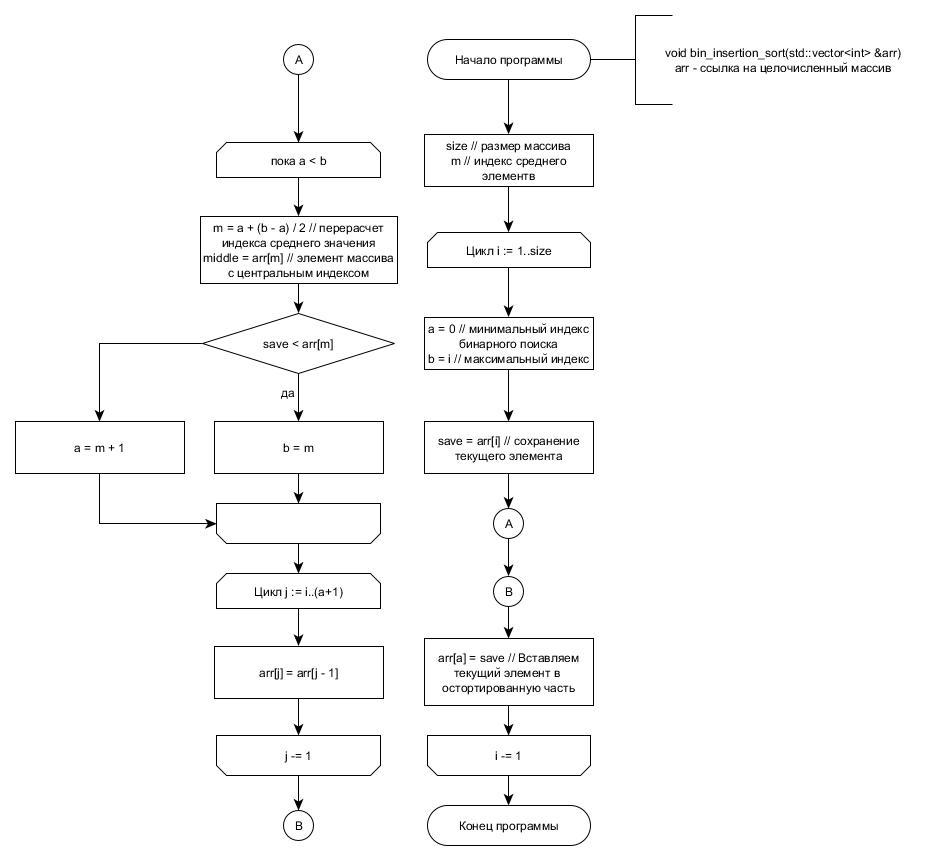
\includegraphics[scale=0.5]{bin_insertion.jpg}
\caption{Функция классического умножения матриц.}
\label{ris:bin_insertion}
\end{figure}

На рисунке \ref{ris:parti_1} показан общий принцип работы(с комментариями!) алгоритма терпеливой сортировки. Детали реализации раскрываются на рисунке \ref{ris:parti_2}.
\begin{figure}[h]
\centering
\center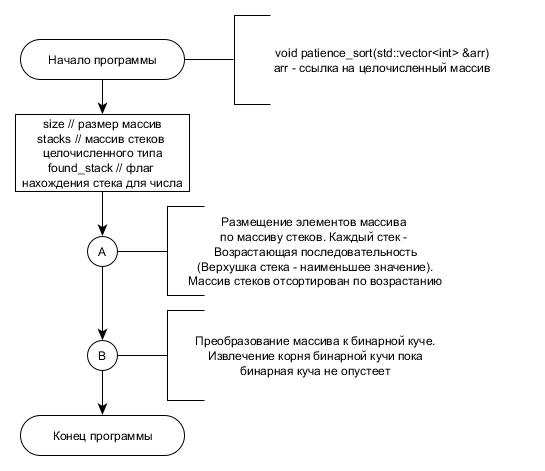
\includegraphics[scale=0.8]{parti_1.jpg}
\caption{Общий принцип работы терпеливой сортировки}
\label{ris:parti_1}
\end{figure}
\begin{figure}[h!]
\centering
\center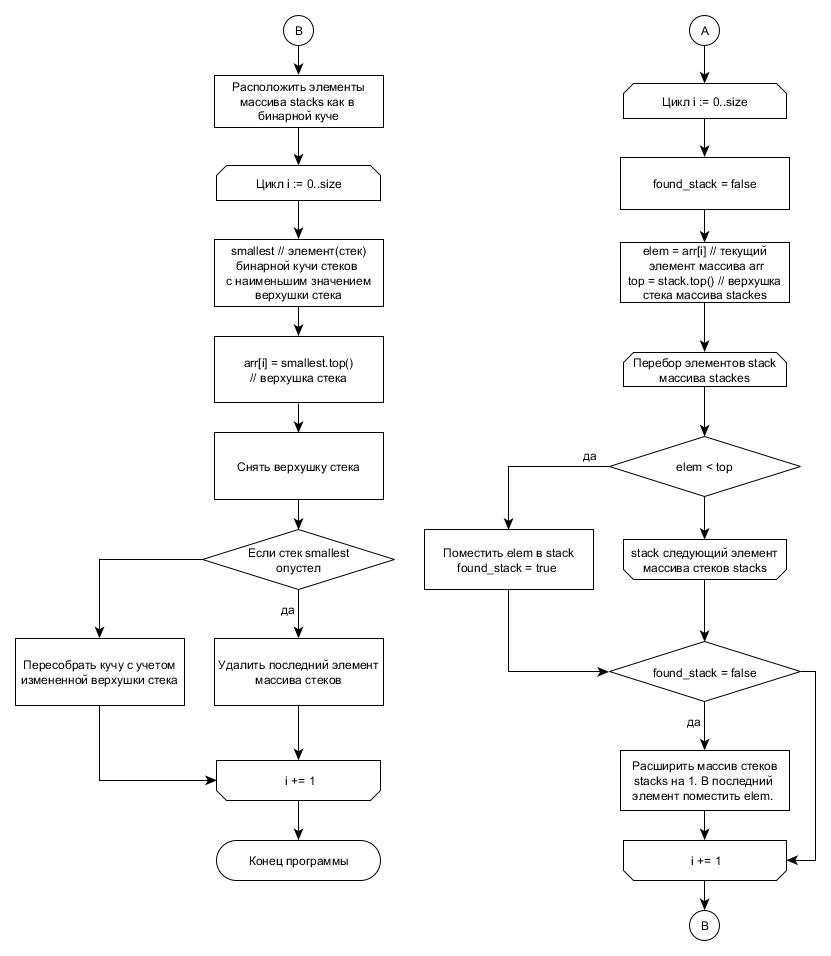
\includegraphics[scale=0.5]{parti_2.jpg}
\caption{Терпеливая сортировка в деталях}
\label{ris:parti_2}
\end{figure}
	
\vspace{300pt}

На рисунке \ref{ris:radix_1} представлен общее представление структуры поразрядной сортировки LSD. На рисунках \ref{ris:radix_2} и \ref{ris:radix_3} в блоке A и E показаны циклы, корректирующие массив в случае обнаружения отрицательных чисел. в Блоке C и D реализована сортировка подсчетом, лежащая в основе поразрядной сортировки.

\vspace{300pt}
	
\begin{figure}[h!]
\centering
\center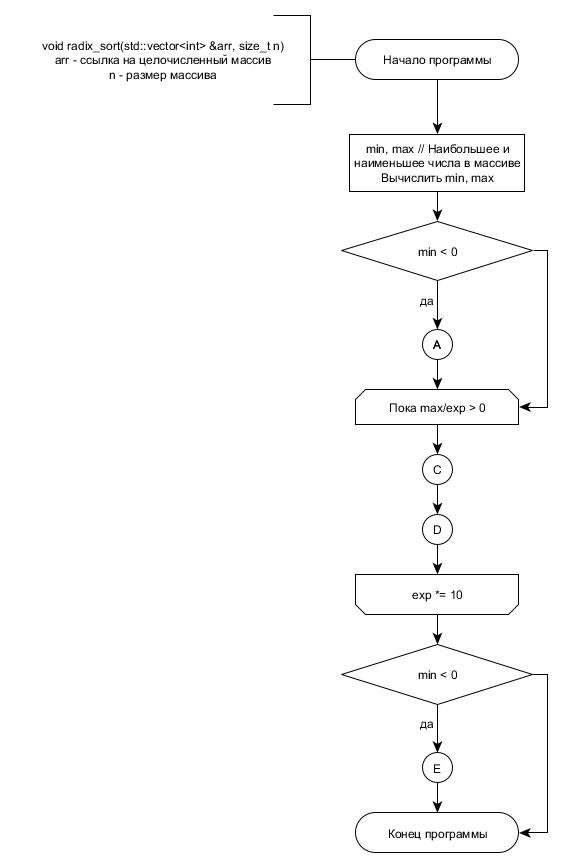
\includegraphics[scale=0.5]{radix_1.jpg}
\caption{Общий принцип поразрядной сортировки LSD}
\label{ris:radix_1}
\end{figure}
\begin{figure}[pt!]
\centering
\center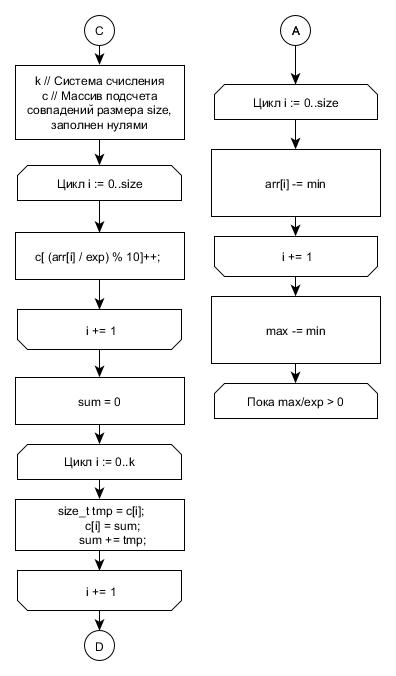
\includegraphics[scale=0.7]{radix_2.jpg}
\caption{Сортировка подсчетом. Часть 1}
\label{ris:radix_3}
\end{figure}
\begin{figure}[pt!]
\centering
\center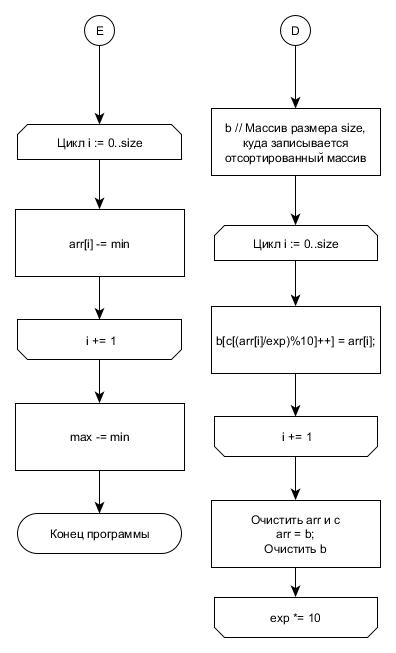
\includegraphics[scale=0.7]{radix_3.jpg}
\caption{Сортировка подсчетом. Часть 2}
\label{ris:radix_2}
\end{figure}
	\newpage
	\section{Технологическая часть}
	\hspace{1cm}В данном разделе будут приведены требования к программнму обеспечению и средства реализации и листинг кода.
	\subsection{Требования к программному обеспечению}
	 \hspace{1cm} Требуется указать размер массива и его элементы.Размер массива должен быть больше нуля. Элементы массива, как и размер, представляют из себя целые числа в диапозоне от -2 147 483 648 до +2 147 483 64.
	\subsection{Средства реализации}
	\hspace{1cm}Для реализации программ я выбрал язык программирования - C++, так как имею опыт работы на нём. Среда разработки - Qt. Замеряется время работы процессора с помощью функции, продемонстрированной в листинге \ref{time}.
	\lstset{ %
        language=c++,                 % выбор языка для подсветки (здесь это С)
        basicstyle=\small\sffamily, % размер и начертание шрифта для подсветки кода
        numbers=left,               % где поставить нумерацию строк (слева\справа)
        numberstyle=\tiny,           % размер шрифта для номеров строк
        stepnumber=1,                   % размер шага между двумя номерами строк
        numbersep=-5pt,                % как далеко отстоят номера строк от         подсвечиваемого кода
        backgroundcolor=\color{white}, % цвет фона подсветки - используем         \usepackage{color}
        showspaces=false,            % показывать или нет пробелы специальными     отступами
        showstringspaces=false,      % показывать или нет пробелы в строках
        showtabs=false,             % показывать или нет табуляцию в строках
        frame=single,              % рисовать рамку вокруг кода
        tabsize=2,                 % размер табуляции по умолчанию равен 2 пробелам
        captionpos=t,              % позиция заголовка вверху [t] или внизу [b] 
        breaklines=true,           % автоматически переносить строки (да\нет)
        breakatwhitespace=false, % переносить строки только если есть пробел
        escapeinside={\%*}{*)},   % если нужно добавить комментарии в коде
	    keywordstyle=\color{blue}\ttfamily,
	    stringstyle=\color{red}\ttfamily,
	    commentstyle=\color{green}\ttfamily,
	    morecomment=[l][\color{magenta}]{\#},
	    columns=fullflexible
    }
	\begin{lstlisting}[label=time,caption=Функция замера процессороного времени]
    unsigned long long tick(void)
    {
        unsigned long long d;
        __asm__ __volatile__ ("rdtsc" : "=A"     (d));
        return d;
    }
	\end{lstlisting}
	Эта функция в отличие от встроенной функции таймера, способна считать реальное процессорное время работы программы в тиках\cite{lom}.

	\newpage
	\subsection{Реализация алгоритмов}
	
	В листинге \ref{bin_ins} представлена реализация сортировки вставками с бинарным поиском.
	
	\begin{lstlisting}[label= bin_ins,caption=Сортировка вставками с бинарным поиском]
   void bin_insertion_sort(std::vector<int> &arr) {
        size_t size = arr.size();
        size_t m = 0;
        for (size_t i = 1; i < size; i++) {
            size_t a = 0;
            size_t b = i;
            int save = arr[i];
    
            while (a < b) {
                m = a + (b - a) / 2;
                if (save < arr[m]) {
                    b = m;
                } else {
                    a = m + 1;
                }
            }
            for (size_t j = i; (j > a); j--) {
                arr[j] = arr[j - 1];
            }
            arr[a] = save;
        }
    }
	\end{lstlisting}
	
	
	\newpage
	В листинге \ref{patience} представлена реализация терпеливой сортировки. Для ее реализации были написаны дополнительные структуры moreStack и lessStack, которые необходимы для использования функций бинарной кучи библиотеки STL, продемонстрированная в листинге \ref{compare}.
	
	\begin{lstlisting}[label=patience,caption=Терпеливая сортировка]
       void patience_sort(std::vector<int> &arr, size_t size) {
            std::vector<std::stack<int>> stacks; // массив стеков
        
            typedef std::vector<std::stack<int>>::iterator Iterator;
        
            for (auto it = arr.begin(); it != arr.end(); it++)
            {
                std::stack<int> stack;
                stack.push(*it);
                Iterator iter = std::lower_bound(stacks.begin(), stacks.end(), stack,
                                     lessStack());
                if (iter == stacks.end())
                    stacks.push_back(stack);
                else
                    iter->push(*it);
            }
        
            // Превратить массив стеком в контейнер
            std::make_heap(stacks.begin(), stacks.end(), moreStack());
            for (size_t i = 0; i < size; i++) {
                // Первый стек становится последним, остальные перестраиваются под кучу
                std::pop_heap(stacks.begin(), stacks.end(), moreStack());
                // Достаем последний стек, который на самом деле имеет наибольший приоритет
                
                std::stack<int> &smallest = stacks.back();
                // На верху стека лежит наименьшее число, а до этого был выбран стек с
                // наибольшим приоритетом(наименьшей верхушкой)
                
                arr[i] = smallest.top();
                smallest.pop();
                
                if (smallest.empty()) {
                    stacks.pop_back();
                } 
                else {
                    // Поскольку последний стек обновился, надо пересобрать кучу, имитируя
                    // вставку нового элемента. push_heap "вставляет" последний элемент
                    std::push_heap(stacks.begin(), stacks.end(), moreStack());
                }
            }
        }
	\end{lstlisting}
	
	\begin{lstlisting}[label=compare,caption=Структуры lessStack и moreStack]
    struct moreStack{
        bool operator()(std::stack<int> s1, std::stack<int> s2) {
            return s1.top() > s2.top();
        }
    };
    
    struct lessStack{
        bool operator()(std::stack<int> s1, std::stack<int> s2) {
            return s1.top() < s2.top();
        }
    };

	\end{lstlisting}
	
		В листинге \ref{radix} представлена реализация LSD поразрядной сортировки. Для ее реализации были написаны несколько дополнительных функций. Так, функция из листинга \ref{add} реализует возможность работы данной сортировки с отрицательными числами. А функция get из \ref{get} определяет минимальное и максимальное значения массива для определения наличия отрицательных чисел(по минимальному числу) и количество разрядов, требуемых для обхода(по максимальному числу). И замыкает перечисление функций сортировка подсчетом из листинга \ref{count}, лежащая в основе работы любой поразрядной сортировки.
	
	\begin{lstlisting}[label=radix,caption=Поразрядная LSD сортировка]
        void radix_sort(std::vector<int> &arr, size_t n) {
            int min = 0, max = 0;
            get_min_max_numbers(arr, n, min, max);
            if (min < 0) {
               add_to_all(arr, -min);
               max -= min;
            }
            for (int exp = 1; max/exp > 0; exp *= 10) {
                counting_sort(arr, n, exp);
            }
            if (min < 0) {  
                add_to_all(arr, min); 
            }
        }
	\end{lstlisting}
	\begin{lstlisting}[label=add,caption=Функция прибавляющая число к каждому элементу массива]
        void add_to_all(std::vector<int> &arr, int num) {
            size_t n = arr.size();
            for(size_t i = 0; i < n; ++i ) {
                arr[i] += num;
            }
        }
	\end{lstlisting}
	\begin{lstlisting}[label=get,caption=Функция получающая минимум и максимум в массиве]
        void get_min_max_numbers(std::vector<int> arr, size_t size,
                                 int &min, int &max) {
            min = max = arr[0];
            for (size_t i = 1; i < size; i++) {
                if (arr[i] > max) {
                    max = arr[i];
                } else if (arr[i] < min){
                    min = arr[i];
                }
            }
        }
	\end{lstlisting}
	
		\begin{lstlisting}[label=count,caption=Сортировка подсчетом]
           void counting_sort(std::vector<int> &arr,
                       size_t size, int exp) {
            size_t k = 10;
            std::vector<size_t> c(k, 0);
            for(size_t i = 0; i < size; ++i )
                c[ (arr[i] / exp) % 10]++; ;
            size_t sum = 0;
            for(size_t i = 0; i < k; ++i ) {
                size_t tmp = c[i];
                c[i] = sum;
                sum += tmp;
            }
            std::vector<int> b(size);
            for( size_t i = 0; i < size; ++i ) {
                b[c[(arr[i]/exp)%10]++] = arr[i];
            }
            arr.clear();
            c.clear();
            arr = b;
            b.clear();
        }
	\end{lstlisting}
	


    \newpage
	\section{Экспериментальная часть}
	\hspace{1cm}В данном разделе будут приведена сложность реализованных алгоритмов и их сравнительный анализ на основе экспериментальных данных.
	\subsection{Сложность}
        
        \begin{doublespace}
        \large
        \textbf{Сортировка вставками с бинарным поиском}
        \normalsize
        \end{doublespace}
        
        \hspace{1cm}Для того, чтобы наглядно показать сложность алгоритма сортировки вставками с бинарным поиском приведу листинг кода \ref{bin_ins_code}, из которого видно, что в общем случае сложность равна 2 + 1 + 2 + (size - 1)(2 + 1 + 1 + 2 + 1 + log(i) * (1 + 7 || 8) + 2 + size2(2 + 4)) или же
        12*size -7 + 9*log((n)!) + 6*size*size2. Трудность вызывает 4*size*size2, поскольку size2 зависит от поступающего на вход массива, поэтому предлагается рассмотреть отдельные 2 случая:лучший и худший.
       
        \begin{doublespace}
        \large
        \textbf{Лучший случай}
        \normalsize
        \end{doublespace}
        
        Пусть на вход пришёл массив [1,2,3,4,5,6,7,8]. на первой итерации перед заходом в цикл(16-ая строчка), i = 1, a = 1, size2 = a - i = 0, аналогично на второй итерации, третьей и т.д. Это связано с тем, что мы хотим вставить элемент в то место, в котором он уже находится, поэтому size2 каждый раз будет равняться нулю
    	и общая сложность становится следующей: -7 + 84 + 9log(8!) или \textbf{O(log(n!))} для лучшего случая
    	
    	 \begin{doublespace}
        \large
        \textbf{Худший случай}
        \normalsize
        \end{doublespace}
        
        Пусть на вход пришёл массив [8,7,6,5,4,3,2,1]. На первой итерации i = 1, a = 0, size2 = 1, на второй i = 2, a = 0, size2 = 2 и т.д. На каждой итерации a = 0, поскольку крайний левый элемент неотсортированной части каждый раз меньше всех элементов отсортированной части, поэтому size2 будет n!. Общая сложность: -7 + 84 + 9log(8!) + 6*8*8! или \textbf{O($n^2$)} для худшего случая
    	\begin{lstlisting}[label= bin_ins_code,caption=Сортировка вставками с бинарным поиском]
    	//
        // Модель
        //'/ ','<', '=', '[]', '++', '--', '.'
        // стоимость 1
        //
       void bin_insertion_sort(std::vector<int> &arr) {
        size_t size = arr.size(); //2 +
        size_t m = 0; //1 +
        for (size_t i = 1; i < size; i++) { // 2 + (size-1) * ( 2 +
            size_t a = 0; // 1 +
            size_t b = i; // 1 +
            int save = arr[i]; // 2 +
    
            while (a < b) { // 1 + log(i) * (1 +
                m = a + (b - a) / 2; // 4 +
                if (save < arr[m]) { // 2 + (1 || 2))
                    b = m;
                } else {
                    a = m + 1;
                }
            } // int size2 = i - a
            for (size_t j = i; (j > a); j--) { // 2 + size2 * (2 +
                arr[j] = arr[j - 1]; // 4)
            }
            arr[a] = save; // + 1)
        }
    }
	\end{lstlisting}
	
	 \begin{doublespace}
    \large
    \textbf{Терпеливая сортировка}
    \normalsize
    \end{doublespace}
    
    Создадим список стеков для хранения стопок. При раскладывании элементов по стопкам для поиска самой левой подходящей стопки используем бинарный поиск. Соответственно, поиск самой левой стопки занимает O(log p), где p — количество стопок (стеков). Таким образом, временная сложность раскладывания по стопкам не превышает O(nlogn).

    Для получения отстортированного массива используем бинарную кучу. На каждом шаге алгоритма необходимо извлечь из кучи стек с минимальной вершиной за O(log p), где p — количество стеков в куче. Снять вершину выбранного стека и вернуть его в кучу за O(log p). Получение отсортированного массива займёт O(nlog n) времени. Получение наибольшей возрастающей подпоследовательности выполняется за O(n) по описанному выше алгоритму. Таким образом, алгоритм сортировки требует   \textbf{O(nlogn)} времени \textbf{в худшем случае} и \textbf{O(n) дополнительной памяти} при \textbf{любом} раскладе\cite{parti_state}. В \textbf{лучшем} же случае сложность \textbf{O(N)} \cite{parti_state_best}.
    
    \begin{doublespace}
    \large
    \textbf{Поразрадная LSD сортировка}
    \normalsize
    \end{doublespace}
    Сначала отсортируем их по первому(старшему) разряду. Сортировка в таком случае выполняется с помощью сортировки подсчетом (count sort). Сложность — o(n). Мы получили 10 «корзин» — в которых старший разряд 0, 1, 2 и т.д. Далее в каждой из корзин запускаем ту же процедуру, но только рассматриваем уже не старший разряд, а следующий за ним, и т.д.

    Шагов столько, сколько разрядов в числах. Соответственно, сложность алгоритма — O(n*k), k — число разрядов. \cite{habr}

    
    \newpage    
    \subsection{Сравнительный анализ}
    \hspace{1cm}Для экспериментов использовались массивы, размер которых варьируется от 1000 до 1000 с шагом 1000. 
    Количество повторов каждого эксперимента = 100. Результат одного эксперимента рассчитывается как
    средний из результатов проведенных испытаний с одинаковыми входными данными. Каждая таблица состоит из 4-ёх столбцов. Первый столбец представляет собой количество элементов. Оставшиеся три - время, затраченное в худшем, обычном и лучшем вариантах. Под обычным вариантом подразумевается сортировка массива из случайных чисел. 
    В таблице \ref{tab:bin_ins_sort} приведены результаты замера сортировки вставками с бинарным поисков. Здесь лучший случай, когда массив был отсортирован заранее. Худший же, когда массив обратно-отсортированный. Замеры терпеливой сортировки показаны в таблице \ref{tab:parti_sort}. Лучший случай, когда таблица обратно отсортирована, худший, когда прямо. Результаты работы LSD сортировки можно увидеть в таблице \ref{tab:lsd_sort}. Так как эта сортировка зависит от количества разрядов, то лучший случай, когда разряд всего 1. За обычный случай принята ситуация, когда максимальное количество разрядов равно трём. Худший случай, когда числа отрицательные и количество разрядов равно максимально допустимому в рамках выбранного типа. 
     
    \begin{table}[h]
        \caption{Результаты замеров сортировки вставками с бинарным поиском.}
            \begin{tabular}{ | c | c | c | c | }
                \hline
                 Количество   &  Отсортированный   &  Из случайных чисел  &  Обратно-отсортированный \\
                 элементов &  (в тиках) & (в тиках) & (в тиках) \\ \hline  
                   1000 &    206514  &    8145084   &    15627474  \\
                    2000 &    385240  &    23286510  &    41709682  \\
                    3000 &    463698  &    44311186  &    69365279  \\
                    4000 &    624200  &    60320225  &    118394474 \\
                    5000 &    726015  &    92174428  &    185447617 \\
                    6000 &    851555  &    131531028 &    267783319 \\
                    7000 &    1087951 &    183235489 &    365067903 \\
                    8000 &    1239921 &    239472118 &    479276444 \\
                    9000 &    1438931 &    296470986 &    597333496 \\
                    10000&    1611345 &    373288185 &    748708369 \\
                \hline
            \end{tabular}
        \label{tab:bin_ins_sort}
    \end{table}
     \begin{table}[h]
        \caption{Результаты замеров терпеливой сортировки}
            \begin{tabular}{ | c | c | c | c | }
                \hline
                 Количество   &  Отсортированный   &  Из случайных чисел  &  Обратно-отсортированный \\
                 элементов &  (в тиках) & (в тиках) & (в тиках) \\ \hline  
                     1000 &    26969365  &    20183614   &     7555004  \\
                    2000 &    41837848  &    30510740   &     11882920 \\
                    3000 &    58297726  &    43699749   &     15566613 \\
                    4000 &    73692411  &    57359246   &     20776705 \\
                    5000 &    101998422 &    77268127   &     26669980 \\
                    6000 &    118373450 &    90142691   &     31857210 \\
                    7000 &    135697894 &    104254801  &     36132328 \\
                    8000 &    156642849 &    120577387  &     42425616 \\
                    9000 &    201309386 &    141705472  &     48113387 \\
                    10000&    220771653 &     158540637 &     53537901 \\
                \hline
            \end{tabular}
        \label{tab:parti_sort}
    \end{table}
    \begin{table}[h]
        \caption{Результаты замеров поразрядной LSD сортировки}
            \begin{tabular}{ | c | c | c | c | }
                \hline
                 Количество   &  Из случайных чисел   &  Из случайных чисел  &  Из отрицательных чисел \\
                 элементов &  от 0 до 10(в тиках) & от 0 до 1000(в тиках) & больших -1000000 (в тиках) \\ \hline  
                    1000 &    124241   &  314779  &    808965 \\
                    2000 &    235804   &  549783  &    1447132\\
                    3000 &    344252   &  744940  &    2094131\\
                    4000 &    416376   &  1094003 &    2894579\\
                    5000 &    527703   &  1333514 &    3421013\\
                    6000 &    653100   &  1616399 &    4800591\\
                    7000 &    720129   &  1988292 &    5213457\\
                    8000 &    810016   &  2116511 &    5743089\\
                    9000 &    890413   &  2411941 &    6521953\\
                    10000&    1062303  &  2724617 &    7134253\\
                \hline
            \end{tabular}
        \label{tab:lsd_sort}
    \end{table}
    
    \newpage
   Ниже приведены графики, на которых наглядно видна сравнительная скорость работы обсуждаемых алгоритмов. Смотрите на графики \ref{grf:best_gr}, \ref{grf:usual_sort} и \ref{grf:lsd}.
 
    
    \begin{figure}
        \centering
        \includegraphics{}
       
    \begin{tikzpicture}
		\begin{axis}[
		    %title = ..  График лучших случаев сортировок,
		    xlabel={Размерность массива},
		    ylabel={Время в тиках},
		    ymin = 0, ymax = 5353790,
		    legend pos=north west,
		    ymajorgrids=true,
		    grid style=dashed,
		]
		\legend{ 
	        Бинарные вставки, 
	        Терпеливая, 
	        Поразрядная
	        }
  		\addplot[
  		    color=red,
  		    mark=square,
  		    ]
  		   coordinates {
  		    (1000,206514)
  		    (2000,385240)
  		    (3000,463698)
  		    (4000,624200)
			(5000,726015)
			(6000,851555)
			(7000,1087951)
			(8000,1239921)
			(9000,1438931)
			(10000,1611345)
  		    };

		\addplot[
  		    color=blue,
  		    mark=square,
  		    ]
  		    coordinates {
  		    (1000,755500)
  		    (2000,1188292)
  		    (3000,1556661)
  		    (4000,2077670)
			(5000,2666998)
			(6000,3185721)
			(7000,3613232)
			(8000,4242561)
			(9000,4811338)
			(10000,5353790)
  		    };
  		    
  	    \addplot[
  		    color=green,
  		    mark=square,
  		    ]
  		    coordinates {
  		    (1000,124241)
  		    (2000,235804)
  		    (3000,344252)
  		    (4000,416376)
			(5000,527703)
			(6000,653100)
			(7000,720129)
			(8000,810016)
			(9000,890413)
			(10000,1062303)
  		    };
		\end{axis}
	\end{tikzpicture}
	 \caption{График лучших случаев сортировок}
        \label{grf:best_gr}
    \end{figure}   
    
    \begin{figure}
        \centering
        \includegraphics{}
        
	 \begin{tikzpicture}
		\begin{axis}[
		    %title = ...  График обычных случаев сортировок,
		    xlabel={Размерность массива},
		    ylabel={Время в тиках},
		    ymin = 0, ymax = 373288185,
		    legend pos=north west,
		    ymajorgrids=true,
		    grid style=dashed,
		]
		\legend{ 
	        Бинарные вставки, 
	        Терпеливая, 
	        Поразрядная
	        }
  		\addplot[
  		    color=red,
  		    mark=square,
  		    ]
  		   coordinates {
  		    (1000,8145084)
  		    (2000,23286510)
  		    (3000,44311186)
  		    (4000,60320225)
			(5000,92174428)
			(6000,131531028)
			(7000,183235489)
			(8000,239472118)
			(9000,296470986)
			(10000,373288185)
  		    };

		\addplot[
  		    color=blue,
  		    mark=square,
  		    ]
  		    coordinates {
  		    (1000,20183614)
  		    (2000,30510740)
  		    (3000,43699749)
  		    (4000,57359246)
			(5000,77268127)
			(6000,90142691)
			(7000,104254801)
			(8000,120577387)
			(9000,141705472)
			(10000,158540637)
  		    };
  		    
  	    \addplot[
  		    color=green,
  		    mark=square,
  		    ]
  		    coordinates {
  		    (1000,314779)
  		    (2000,549783)
  		    (3000,744940)
  		    (4000,1094003)
			(5000,1333514)
			(6000,1616399)
			(7000,1988292)
			(8000,2116511)
			(9000,2411941)
			(10000,2724617)
  		    };

		\end{axis}
	\end{tikzpicture}
	\caption{График обычных случаев сортировок}
        \label{grf:usual_sort}
    \end{figure}
	
	\begin{figure}
	    \centering
	    \includegraphics{}
	 \begin{tikzpicture}
		\begin{axis}[
		    %title = ..  График худших случаев сортировок,
		    xlabel={Размерность массива},
		    ylabel={Время в тиках},
		    ymin = 0, ymax = 748708369,
		    legend pos=north west,
		    ymajorgrids=true,
		    grid style=dashed,
		]
		\legend{ 
	        Бинарные вставки, 
	        Терпеливая, 
	        Поразрядная
	        }
  		\addplot[
  		    color=red,
  		    mark=square,
  		    ]
  		   coordinates {
  		    (1000,15627474)
  		    (2000,41709682)
  		    (3000,69365279)
  		    (4000,118394474)
			(5000,185447617)
			(6000,267783319)
			(7000,365067903)
			(8000,479276444)
			(9000,597333496)
			(10000,748708369)
  		    };

		\addplot[
  		    color=blue,
  		    mark=square,
  		    ]
  		    coordinates {
  		    (1000,26969365)
  		    (2000,41837848)
  		    (3000,58297726)
  		    (4000,73692411)
			(5000,101998422)
			(6000,118373450)
			(7000,135697894)
			(8000,156642849)
			(9000,201309386)
			(10000,220771653)
  		    };
  		    
  	    \addplot[
  		    color=green,
  		    mark=square,
  		    ]
  		    coordinates {
  		    (1000,808965)
  		    (2000,1447132)
  		    (3000,2094131)
  		    (4000,2894579)
			(5000,3421013)
			(6000,4800591)
			(7000,5213457)
			(8000,5743089)
			(9000,6521953)
			(10000,7134253)
  		    };

		\end{axis}
	\end{tikzpicture}
	 \caption{График худших случаев сортировок}
	    \label{grf:lsd}
	\end{figure}
	
    \newpage
	\section*{Вывод}
    \addcontentsline{toc}{section}{Вывод}
    
    
	\hspace{1cm}В результате проведенного эксперимента был получен следующий вывод: алгоритм Бинарных вставок справляктся лучше всех в случае, когда массив заранее отсортирован. Поразрядная сортировка лучше всего работает, когда разброс значений(а значит и количество разрядов) не столь велико, однако и в остальных случаях, LSD сортировка ведет очень расторопно - быстрее всех остальных рассмотренных здесь сортировок. Терпеливая сортировка тратит много времени на распределение элементов по стопкам и преобразование массива к бинарной куче, за счет чего не может потягаться с той же поразрядной сортировкой и даже проигрывает вставкам с бинарным поиском в своем лучшем случае.
	\newpage
	\section*{Заключение}
    \addcontentsline{toc}{section}{Заключение}
    
	\hspace{1cm}В ходе работы были изучены и реализованы алгоритмы сортировки вставками с бинарным поиском, терпеливой сортировки и поразрядной. Подтвердилось, что поразрядная сортировка наиболее эффиективная при различных наборах данных. Бинарные вставки не смотря на свою простоту в некоторых случаях(когда массив частично отсортирован) могут потягаться с более продвинутыми своими 'коллегами'. Терпеливую же следует использовать по своему назначению - для поиска наибольшей подпоследовательности в последовательности.
    

    \newpage

    \addcontentsline{toc}{section}{Список литературы}
    \begin{thebibliography}{11} 
    \bibitem{alg_params} Кантор Илья, http://algolist.manual.ru/sort/ 
    \bibitem{alg_list} Российский государственный социальный университет, Кафедра «Финансы и кредит», Великохатько Кира, https://studfiles.net/preview/4652654/
   \bibitem{knut} Кнут Д. Э. 5.2.1 Сортировка путём вставок // Искусство программирования. Том 3. Сортировка и поиск = The Art of Computer Programming. Volume 3. Sorting and Searching / под ред. В. Т. Тертышного (гл. 5) и И. В. Красикова (гл. 6). — 2-е изд. — Москва: Вильямс, 2007. — Т. 3. — 832 с. — ISBN 5-8459-0082-1.
    \bibitem{korman}Кормен, Т., Лейзерсон, Ч., Ривест, Р., Штайн, К. 2.1. Сортировка вставкой // Алгоритмы: построение и анализ = Introduction to Algorithms / Под ред. И. В. Красикова. — 3-е изд. — М.: Вильямс, 2013. — С. 38-45. — ISBN 5-8459-1794-8.
     \bibitem{macconel} Макконнелл Дж. Основы современных алгоритмов = Analysis of Algorithms: An Active Learning Approach / Под ред. С. К. Ландо. — М.: Техносфера, 2004. — С. 72-76. — ISBN 5-94836-005-9.
    \bibitem{lom}И.В. Ломовской. Курс лекций по языку программирования C, 2017
    \bibitem{parti_state} Университет ИТМО, статья про терпеливую сортировку, http://neerc.ifmo.ru/wiki/index.php?title=Терпеливаясортировка
   
    \bibitem{parti_state_best} Chandramouli, Badrish; Goldstein, Jonathan (2014). Patience is a Virtue: Revisiting Merge and Sort on Modern Processors (PDF). SIGMOD/PODS. 
    
    \bibitem{habr}https://habr.com/post/268261/
    
    \end{thebibliography}

\end{document}